%-----------------------------------------------------------------------
% Cabecera del documento. Aqui se incluyen los paquetes y las
% definiciones que se utilizen despues en el documento.

\documentclass[a4paper,11pt]{article} % Tipo del documento. Puede ser
                                      % book, article, report, y
                                      % muchos mas

\usepackage{./estilos/estiloBase} % Basicamente son todas las
                                  % librerias usadas. En caso de que
                                  % falten librerias se van añadiendo
                                  % al fichero.
\usepackage{./estilos/colores}  % Algunos colores ya generados, para
                                % los algunos estilos más avanzados.
\usepackage{./estilos/comandos} % Algunos comandos personalizados

%\usepackage{./estilos/pygments}

\graphicspath{{./imagenes/}}

\title{Zycars: juego de conducción en 2D} % Título del documento
\author{Alumno: José Jesús Marente Florín\\Directores: Manuel Palomo Duarte y Juan Manuel Dodero Beardo} % Autor (o
                                 % autores)
\date{\today} % Fecha. La orden \today indica el dia de hoy con dia
              % mes y año. 

%----------------------------------------------------------------------

\begin{document} % Lo que este en el entorno document es lo que se va
                 % a mostrar finalmente.
%\sinmargen
\maketitle % Generacion automatica del titulo o la portada si es un book.

\abstract{\noindent El siguiente documento se presenta a modo de resumen que
  complementa la Memoria del mismo Proyecto Fin de Carrera, entregada de forma
  simultánea a este resumen. El proyecto consiste en un videojuego de conducción
  en dos dimensiones.}

\tableofcontents % Genera automaticamente el indice. Es necesario
                 % compilar dos veces para que este salga.

%%%%%%%%%%%%%%%%%%%%%%%%%%%%%%%%%%%%%%%%%%%%%%%%%%%%%%%%%%%%%%%%%%%%%%%%%%%%%%%
%%%%%%%%%%%%%%%%%%%%%%%%%%%%%%%%OBJETIVOS%%%%%%%%%%%%%%%%%%%%%%%%%%%%%%%%%%%%
%%%%%%%%%%%%%%%%%%%%%%%%%%%%%%%%%%%%%%%%%%%%%%%%%%%%%%%%%%%%%%%%%%%%%%%%%%%%%%%
\section{Objetivos}

\paragraph{}
El objetivo del proyecto es realizar un videojuego de conducción en dos dimensiones con vista cenital\footnote{Los elementos son
vistos desde arriba}. Se podría decir que el juego tendrá tintes de juegos como Micro Machines, disponible para diversas 
plataformas, y del Mario Kart de nintendo.

\paragraph{}
Otro de los objetivos principales del proyecto, es la realización del juego tanto para personas que
dedican varias horas a la consecución de videojuegos, tanto para personas casuales, que dedican poco tiempo
jugando.

\paragraph{}
Por lo que ser un juego de conducción el cual no esta compuesto por ninguna historia o trama argumental, facilita que se le pueda
dedicar pequeños intervalos de tiempo o, sin embargo, dedicarle varias horas al día.

\paragraph{}
Otro de los objetivos del proyecto, es poder hacerlo ampliable, de forma que cualquier persona mediante indicaciones y manuales
pueda añadir tanto nuevos personajes, como circuitos en los que competir.

\section{Motivaciones}

\paragraph{}
Mi interés por el mundo de los videojuegos, desde muy pequeño, y tras haber cursado en la carrera
la asignatura optativa de "Diseño de videojuegos", donde aprendí mucho
relacionado con el desarrollo de estos,
aumentó mi interés por este mundo y además el desarrollo de ellos. Por lo que desde entonces consideraba seriamente realizar 
como proyecto fin de carrera un videojuego.

\paragraph{}
También he de añadir que tras conocer abiertamente el mundo del Software libre, gracias a la importancia que se le presta
en la Universidad de Cádiz. Se decidió que el proyecto fuera software libre bajo licencia GPL 3. Y así cualquier persona
interesada en el desarrollo de videojuegos y en el software libre en general, pudiera usar los recursos del proyecto
libremente.

%%%%%%%%%%%%%%%%%%%%%%%%%%%%%%%%%%%%%%%%%%%%%%%%%%%%%%%%%%%%%%%%%%%%%%%%%%%%%%%
%%%%%%%%%%%%%%%%%%%%%%%%%%%%%%%PLANIFICACION%%%%%%%%%%%%%%%%%%%%%%%%%%%%%%%%%%%
%%%%%%%%%%%%%%%%%%%%%%%%%%%%%%%%%%%%%%%%%%%%%%%%%%%%%%%%%%%%%%%%%%%%%%%%%%%%%%%
\section{Planificación}

\paragraph{}
La planificación realizada para el desarrollo del proyecto, está dividida en varias partes:

%\begin{itemize}
%    \item \textbf{Fase inicial}: la primera fase consistió en plantear la idea del proyecto, con la ayuda del tutor. Tras varias
%    propuestas realizadas y la deliveración sobre las mismas, se decidió realizar este proyecto.
%    
%    \item \textbf{Fase de análisis}: durante esta etapa se realizó la especificación de los requisitos
%    \item \textbf{}:
%    \item \textbf{}:
%    \item \textbf{}:
%    \item \textbf{}:
%\end{itemize}

\subsection{Fase inicial}

\paragraph{}
La primera fase consistió en plantear la idea del proyecto, con la ayuda del tutor. Tras varias
propuestas y la deliberación sobre las mismas, se decidió realizar este proyecto.

\paragraph{}
También se pensó en que lenguaje se desarrollaría el proyecto, así como las principales bibliotecas
que se usarían durante la realización del mismo.

\subsection{Fase de análisis}

\paragraph{}
Esta etapa está dividida principalmente en las dos partes siguiente:

\begin{itemize}
    \item \textbf{Especificación de los requisitos}: estudio de los requisitos que deberá cumplir el juego.
    
    \item \textbf{Recurso necesarios}: recursos necesarios que deberemos usar durante el desarrollo del proyecto.
\end{itemize}

\subsection{Fase Aprendizaje}

\paragraph{}
Dado que el proyecto se realizaría con un lenguaje de programación del que no se tenían conocimientos, en este caso \emph{Python}, 
así como de la biblioteca que usaríamos en el desarrollo, como es \emph{Pygame}, esta fase se dividió en dos partes:

\begin{itemize}
    \item \textbf{Aprendizaje de \emph{Python}}: periodo empleado para el aprendizaje del lenguaje de programación \emph{Python},
    durante esta etapa se consultó varios libros sobre lenguaje, así como foros de internet y páginas web. Para un aprendizaje más
    ameno y llevadero, se realizaron problemas ya resuelto en otros lenguajes.
    
    \item \textbf{Familiarización con la biblioteca \emph{Pygame}}: tras el periodo de aprendizaje del lenguaje, debía familiarizarme
    con la biblioteca principal que se usaría en el desarrollo del proyecto, como es \emph{Pygame}. Durante su
    aprendizaje se realizaron pequeñas aplicaciones sencillas, para asentar
    bien los conocimientos.
\end{itemize}

\subsection{Fase de desarrollo}

\paragraph{}
Tras la consecución de las etapas anteriores, se comenzó el desarrollo del proyecto. Esta etapa del desarrollo es la más extensa de 
todas, como es comprensible. Y también la etapa que más subetapas contiene, las principales son la siguientes:

\begin{itemize}
    \item \textbf{Motor básico}: implementación de las necesidades básicas del proyecto, como control del teclado, carga de recursos, movimiento
    de los vehículos.
    
    %\item \textbf{Movimiento de vehículos}: relización del movimiento y comportamiento que deberían tener los vehículos: giro, 
    %aceleración, frenada.
    
    \item \textbf{Carga de escenario}: carga de los circuitos que compondrán el juego de forma que no fuera necesario tocar código
    para la ampliación del juego.
    
    \item \textbf{Creación de menús}: implementación de toda la interfaz de menús de la que estaría compuesto el juego, menú de 
    opciones, selección de personaje, selección de circuito, etc.
    
    \item \textbf{Colisiones}: unos de los aspectos más básico y esenciales de cualquier juego, se debía implementar las colisiones con el
    escenario, así como con otros elementos del juego como pueden ser ítems u otros vehículos.
    
    \item \textbf{Ítems}: implementación del comportamiento y efecto que
    producirían cada uno de los ítems que están disponibles en el juego.
    
    \item \textbf{Inteligencia artificial}: planteamiento y desarrollo de los vehículos que serían manejados por la inteligencia 
    artificial, estos deberían de se capaces de evitar obstáculos, realizar
    recorridos y lanzar ítems.
    
    \item \textbf{Modos de juego}: realización de los modos de juego que componen el proyecto, como serían carrera rápida, contrarreloj
    y campeonato,
\end{itemize}

\subsection{Pruebas y correcciones}

\paragraph{}
Una de las etapas más importantes, si no es la que más, del desarrollo de cualquier proyecto. Esta etapa se realizaría en paralelo
a la de desarrollo, ya que conforme se implementan nuevas funcionalidades, cada
un debía ser probada exhaustivamente en cualquiera
de las posibles situaciones que pudiera suceder.

\subsection{Redacción de la memoria}

\paragraph{}
La redacción de la memoria se ha redactado conforme se iba avanzando en el desarrollo del proyecto. Pero tras la finalización
de este, se le ha dedicado más tiempo a la finalización de la memoria.

\subsection{Diagrama de Gantt}

\paragraph{}
Diagrama de Gantt de la planificación comentada (Figura \ref{fig:gant1} y \ref{fig:gant2})

%%%%%%%%%%%%%%%%%%%%%%%%%%%%%%%%%%%%%%%%%%%%%%%%%%%%%%%%%%%%%%%%%%%%%%%%%%%%%%%
%%%%%%%%%%%%%%%%%%%%%%%%%%%%%%%%DESCRIPCION%%%%%%%%%%%%%%%%%%%%%%%%%%%%%%%%%%%%
%%%%%%%%%%%%%%%%%%%%%%%%%%%%%%%%%%%%%%%%%%%%%%%%%%%%%%%%%%%%%%%%%%%%%%%%%%%%%%%
\section{Descripción general}

\paragraph{}
El proyecto consiste en un juego de carreras en dos dimensiones con vista cenital, en el que se podrá competirá contra la 
inteligencia artificial. 

\begin{figure}[H]
  \label{logo_zycars}
  \begin{center}
    
\includegraphics[scale=0.5]{imagenes/logo_zycars.png}
  \end{center}
  \caption{Logo de Zycars}
\end{figure}

\subsection{Características del videojuego}

\paragraph{}
El videojuego ofrece una alternativa libre, gratuita y original para jugar a un juego de conducción en dos dimensiones. 
Las posibilidades que ofrece son las siguientes:

\subsubsection{Modos de juego}

\paragraph{}
En \emph{Zycars} tendremos distintos modos de juegos, en cada uno de ellos el
objetivo que habrá que llevar a cabo será distinto.
A continuación se describirán los distintos modos de juegos que tendrá el videjuego:

\begin{description}

\item[Carrera rápida]
El juego en el modo de carrera rápida ofrece la posibilidad de enfrentarnos a 3 personajes 
controlados por la inteligencia artificial, a lo largo de un circuito que
hayamos seleccionado previamente. El número de vueltas
que se realicen durante la carrera estarán a elección del jugador y se podrá elegir el número de las mismas a la hora de seleccionar
el circuito.

\item[Campeonato]
En este modo de juego podremos competir contra 3 personaje controlados por la inteligencia artificial 
a lo largo de un campeonato completo, el cual habremos elegido previamente. 

El campeonato estará compuesto por cuatro circuitos y el número de vueltas a estos, también estarán a elección del jugador 
al igual que en el modo de juego explicado anteriormente.

Tras la conclusión de cada una de las carreras, los jugadores obtendrán una puntuación en función de la posición que haya 
obtenido. El jugador que mayor puntuación haya conseguido tras acabar los cuatro circuitos, se proclamará ganador del 
campeonato.

\item[Contrarreloj]
En este último modo de juego y a diferencia de los dos anteriores, el jugador competirá solo sin ningún oponente.

El objetivo en este modo de juego será la realización de los circuitos ofrecidos y mejorar los tiempos de estos, ya sean la 
vuelta más rápida del circuito o el tiempo general. El número de vueltas que deberemos dar al circuito serán un total de tres, a
diferencia de los modos anteriores, no tendremos la posibilidad de modificar el valor.

\end{description}


\subsubsection{Elementos de juego}

\paragraph{}
En esta sección se hará una pequeña descripción de los distintos elementos que encontraremos a lo largo del juego, ya sean 
manipulados por los jugadores, o encontrados a lo largo de los circuitos.


\begin{description}

\item [Personajes]
Los elementos básico del juego, habrá disponibles distintos personajes que tendrán asociado un 
vehículo característico a su personalidad y apariencia. Cada uno de ellos
tendrán distintas características, 
cosa a tener en cuenta a la hora de hacer nuestra elección por uno de ellos, como la velocidad, la aceleración y el giro.
	
\begin{figure}[H]
	\label{ejemplo_personaje2}
	\begin{center}
		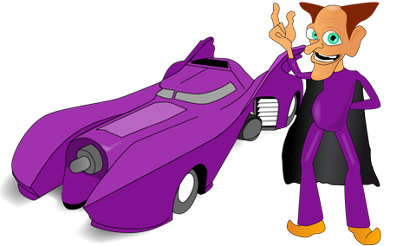
\includegraphics[scale=0.4]{imagenes/ejemplo_personaje2.png}
	\end{center}
	\caption{Personaje de Zycars.}
\end{figure}

\item [Cajas de ítems]
A lo largo de los circuitos en los que estemos compitiendo contra la inteligencia artificial, 
podremos encontrar distintas cajas que al colisionar con ellas nos proporcionen
aleatoriamente una habilidad o ítem que nos
ayuden en la competición contra nuestros rivales.

\begin{figure}[H]
	\label{item_box}
	\begin{center}
		
\includegraphics[scale=0.85]{imagenes/items/item_box.png}
	\end{center}
	\caption{Caja de ítem.}
\end{figure}

\item [Tipos de ítems]

Los ítems que podremos obtener a partir de la caja de ítems, los podremos diferenciar principalmente en tres tipos:

\begin{description}
	\item \textbf{Ataques a distancia} Estos nos permitirán lanzar ataques
        de forma que podamos interceptar a los competidores que 
	se encuentres lejos de nosotros.
	
	\item \textbf{Obstáculos} Estos nos permitan dejar obstáculos en el
        recorrido, que reduzcan nuestra velocidad considerablemente
	o aquellos que al pasar por encima perdamos completamente el control de nuestro vehículo por unos instantes de tiempo.
	
	\item \textbf{Velocidad} Estos nos darán la opción de aumentar nuestra velocidad durante un pequeño intervalo de tiempo.
\end{description}

\end{description}

\subsection{Colaboradores}

\paragraph{}
Todo el apartado del proyecto referente a la programación del mismo se ha realizado de forma individual. En cambio, otros apartados
como el diseño gráfico, se ha contado con la colaboración de otra persona, y la música se ha obtenido de internet, concretamente 
de Jamendo, la página de música libre publicadas bajo licencias Creative Commons. Los créditos de juego son los siguientes:

\begin{description}
    \item [Desarrollador] José J. Marente Florín
    \item [Diseñador Gráfico] David Nieto Rojas
    \item [Música] Bob Wizman, Pirato Ketchup, Los Cadaver, The Wavers, Zamalska 
\end{description}

%%%%%%%%%%%%%%%%%%%%%%%%%%%%%%%%%%%%%%%%%%%%%%%%%%%%%%%%%%%%%%%%%%%%%%%%%%%%%%
%%%%%%%%%%%%%%%%%%%%%%%%%%%%%%IMPLEMENTACION%%%%%%%%%%%%%%%%%%%%%%%%%%%%%%%%%%
%%%%%%%%%%%%%%%%%%%%%%%%%%%%%%%%%%%%%%%%%%%%%%%%%%%%%%%%%%%%%%%%%%%%%%%%%%%%%%
\section{Implementación}

\paragraph{}
Durante todo el desarrollo del proyecto, han ido apareciendo diversas dificultades y problemas que se debieron ir
resolviendo para el correcto y continuo avance del proyecto.

\subsection{Carga desde ficheros}

\paragraph{}
Desde un primer momento se pensó en realizar el videojuego de forma que fuera facilmente ampliable siguiendo un manual adecuado, 
donde se explicaran todos los pasos necesarios .

\paragraph{}
Para ello se optó por realizar toda la carga de circuitos, personajes e interfaces de los menús desde archivos. El formato de 
dichos archivos sería XML.

\paragraph{}
De esta forma cualquier persona ya sea programador o no, podrá modificar aspectos tan sencillos como el posicionamiento de los 
botones en lo menús, y las distintas imágenes que pueden aparecer en estos. Respecto a los personaje podrán modificar las 
características de estos, las imágenes que los representan o añadir nuevos personajes. En los circuitos podremos modificar objetos
que aparezcan en estos, así como obstáculos o aparición de ítems.

\subsection{Formato y carga de circuitos}

\paragraph{}
Una de las primeras dudas que surgieron al poco tiempo de comenzar el desarrollo de \emph{Zycars}, fue el formato que deberían
tener los distintos circuitos o niveles que aparecerían a lo largo del juego. En un principio se barajaron varias alternativas.

\paragraph{}
Finalmente se optó por usar el programa \emph{Tiled}, dicho programa me proporcionaba todas las necesidades básicas, como una 
sencilla edición y creación de niveles, así como la gestión de capas, para poder poner elementos en el circuito a un nivel 
superior o inferior. Para ello se debía crear una imagen con todos los tiles que compondrían un circuito.

\paragraph{}
Una de las únicas cosas que no proporcionaba el programa era poder indicar cuales de los tiles eran colisionables, atravesables o
de cualquier otro tipo. Así que para solventar este problema se eligió tener a parte de la imagen que contendría el conjunto de 
tiles otra imagen con las mismas características, como tamaño y el tamaño de los tiles, solo que esta última, lo tiles tendrían 
colores planos indicando de que tipo serían. Así cuando cargáramos el circuito
que necesitáramos en ese momento y con ello
el conjunto de tiles relacionado, se comprobaría que color tiene cada uno de los tiles en la otra imagen y así almacenar
de que tipo son. A continuación se muestran dos imágenes como ejemplo:

\begin{figure}[H]
  \label{tileset}
  \begin{center}
    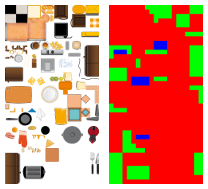
\includegraphics[scale=0.245]{imagenes/tileset-collisionmap.png}
  \end{center}
  \caption{Conjunto de tiles y mapa de colisiones del mismo}
\end{figure}

\subsection{Colisiones}

\paragraph{}
La detección de las colisiones es una de las cosas más básicas de la mayoría de los juegos en la que los jugadores
recorren mapas o niveles.

\subsubsection{Colisión con el escenario}

\paragraph{}
Como se comento en el apartado dedicado a la carga y formato de los circuitos, cada uno de los circuitos tiene asociado una imagen
que indica de que tipo es cada uno de los tiles que nos podemos encontrar a lo largo del circuito.

\paragraph{}
Así que a la hora de cargar el circuito en el que vayamos a competir almacenábamos cada uno de los tiles que componían el circuito,
así como el tipo que eran. Dada esta situación debemos ir comprobando si el jugador esta atravesando algún tile colisionable. 
Si es el caso, debemos corregir la posición del objeto con respecto al tile con el que estaba colisionando.

\paragraph{}
A la hora de realizar la corrección de la colisión, debemos tener en cuenta aspectos como, ángulo del vehículo, dirección del 
vehículo, así como el lado del tile por el que se produce la colisión, ya sea por la parte superior, inferior o alguno 
de los laterales. Según estos parámetros la colisión se corregirá en una dirección u otra.

\paragraph{}
A continuación se muestra un ejemplo visual:

    \begin{figure}[H]
      \label{colision2}
      \begin{center}
        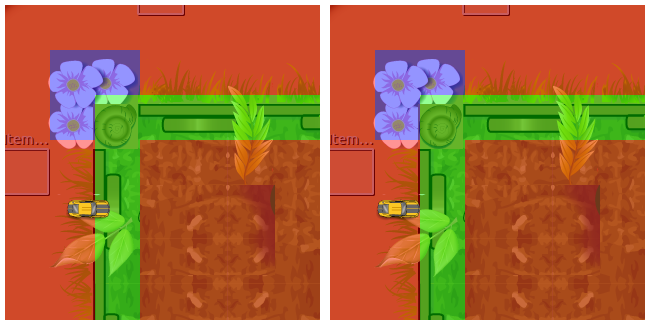
\includegraphics[scale=0.5]{imagenes/colision1-colision2.png}
      \end{center}
      \caption{Colisión con el escenario}
    \end{figure}

\subsubsection{Colisiones entre objetos}

\paragraph{}
En este caso hay varias posibilidades según que tipos de objetos han colisionado, en todas ellas la detección de la colisión
se hace de forma similar, comprobamos si alguna de las caja de colisiones de los objetos en cuestión se superponen o no.

\paragraph{}
A continuación se exponen las distintas situaciones que pueden suceder:

\begin{itemize}
    \item \textbf{Colisión vehículo-vehículo}: dos vehículos en carrera colisionan entre sí, en este caso debemos comprobar 
    cual de los dos vehículos ha colisionado con el otro, es decir, cual se ha interpuesto. En ese caso 
    corregiremos la posición de ese vehículo y produciremos algún tipo de rebote en función de la velocidad que llevara
    en ese momento.
    
    \item \textbf{Colisión vehículo-ítem}: en este caso se responderá a la
    colisión dependiendo del tipo de ítem con el que
    hemos colisionado.
\end{itemize}

\subsection{Inteligencia artificial}

\paragraph{}
Otro de los aspectos más importante de un videojuego de las características de \emph{Zycars}, es la inteligencia artificial,
ya que en dos de los tres modos de juegos disponibles el objetivo es obtener la mejor clasificación posible, por delante
de los demás coches manejados por la inteligencia artificial.

\paragraph{}
Entre las habilidades que debe tener la inteligencia artificial deben ser:

\begin{itemize}
    \item \textbf{Realización del recorrido}: la inteligencia artificial debe ser capaz de realizar los recorridos de los
    circuitos.
    
    \item \textbf{Lanzamiento de ítems}: también debe poder tirar los ítems que
    reciba de las bolas de ítems.
\end{itemize}

\subsubsection{Realización del recorrido. Algoritmo de búsqueda A*}

\paragraph{}
A lo largo de los circuitos existen unos puntos de control que cada uno de los vehículo de la inteligencia artificial
debe pasar para realizar la vuelta al circuito, dichos puntos de control ocupan un tile.

\paragraph{}
Para ello, aprovechando que tenemos un circuito creado por tiles y que podemos
saber en todo momento en el tile actual
que se puede encontrar cualquiera de los competidores, se decidió que se implementaría el algoritmo de búsqueda A*.

\paragraph{}
Dicho algoritmo se aplica en \emph{Zycars}, de forma que el vehículo controlado por la inteligencia artificial, tiene todos los
puntos de chequeo, en orden, que debe atravesar para recorrer el circuito completo. Así que en cada momento se comprobará
el tile actual en el que se encuentra y se obtendrá el camino más óptimo y corto hasta el siguiente punto de chequeo, una vez
llegado a este punto, se hará una nueva consulta al A* para obtener el camino al próximo y así sucesivamente.

\subsubsection{Lanzamiento de ítems.}

\paragraph{}
Como solución, se eligió una forma muy sencilla y eficiente a la hora de realizarlo. Para ello cada vehículo controlado por la
inteligencia artificial, tiene tanto un segmento que va desde el centro del
coche hacia unos píxeles por delante de la posición
actual del vehículo, como otro segmento que también va desde el centro pero uno
píxeles atrás de la posición del vehículo. 
Si se pudieran ver dichos segmentos, tendrían la siguiente forma:

\begin{figure}[H]
  \label{ia_segmentos}
  \begin{center}
    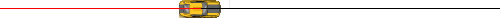
\includegraphics[scale=0.8]{imagenes/ia_segmentos.png}
  \end{center}
  \caption{Segmentos de la inteligencia artificial}
\end{figure}


%%%%%%%%%%%%%%%%%%%%%%%%%%%%%%%%%%%%%%%%%%%%%%%%%%%%%%%%%%%%%%%%%%%%%%%%%%%%%%
%%%%%%%%%%%%%%%%%%%%%%%%%%%%%%%%%TECNOLOGIAS%%%%%%%%%%%%%%%%%%%%%%%%%%%%%%%%%%
%%%%%%%%%%%%%%%%%%%%%%%%%%%%%%%%%%%%%%%%%%%%%%%%%%%%%%%%%%%%%%%%%%%%%%%%%%%%%%
\section{Tecnologías implicadas}

\subsection{Lenguaje de programación}

\paragraph{}
Se decidió usar \emph{Python} como lenguaje principal para el desarrollo de \emph{Zycars}. \emph{Python} es un lenguaje de 
programación interpretado, de alto nivel, usa tipado dinámico, es fuertemente tipado y multiplataforma. Se trata de un lenguaje de 
programación multiparadigma ya que soporta orientación a objetos, programación imperativa y, en menor medida, programación 
funcional. Cabe destacar que se han obtenido unos resultado muy satisfactorios y ha cumplido todas las expectativas esperadas.

\subsection{Biblioteca gráfica}

\paragraph{}
En este caso se tuvo clara la elección desde el momento en el que se decidió usar \emph{Python} como lenguaje principal, me decanté
por la biblioteca gráfica \emph{Pygame}. Dicha biblioteca es un wrapper de la biblioteca \emph{SDL}, de C/C++, para \emph{Python}, 
por lo que tiene todas las virtudes de dicha biblioteca:

\begin{enumerate}
    \item Biblioteca multiplataforma compatible oficialmente con los sistemas Microsoft Windows, GNU/Linux, Mac OS y QNX.
    
    \item Programada en C, por lo que tiene un gran rendimiento.
    
    \item Muy completa, ya que permiten la manipulación tanto de imágenes 2D, como gestión de sonido y música, y también gestión
    de la entrada estándar del sistema. Todos los elementos necesario para el desarrollo de videojuegos.
    
    \item También se usó durante el desarrollo de la asignatura de Diseño de Videojuegos, por lo que se conocen todas sus 
    características muy bien.
\end{enumerate}

\subsection{Analizador de código: Pylint}

\paragraph{}
Se creyó necesario que el código que se implementara siguiera un estándar
uniforme y que estuviera exento de cualquier tipo de 
errores o signos de mala calidad. Para ello se usó la herramienta Pylint.

\paragraph{}
Pylint es una herramienta que analiza el código \emph{Python} en busca de errores y señales de mala calidad. Es una herramienta 
de python que comprueba si un módulo cumple con un estándar de codificación.

\subsection{Sistema de control de versiones}

\paragraph{}
Todo el código y recursos de \emph{Zycars} está alojado en el sistema que proporciona Google Code, que consiste en un entorno completo
usando el sistema de control de versiones \emph{subversion}.

\subsection{Documentación del código}

\paragraph{}
Para la documentación del código me decanté por usar \emph{Doxygen}, esta permite la documentación sencilla y legible de todo el 
código, generando la documentación en varios formatos como puede ser \emph{HTML} o \emph{PDF}.

\paragraph{}
Para python existe la herramienta \emph{Doxypy}, que nos permite usar la convención de comentarios de \emph{Python} y adaptarlos a
\emph{Doxygen}, por lo que nos ahorra trabajo y sigue la normativa de código \emph{Python}.

\subsection{Realización de diagramas: Dia}

\paragraph{}
Dia es un programa de creación de diagramas en GNU/Linux, MacOS X, Unix y Windows, bajo la 
licencia GPL. Puede ser utilizado para dibujar diferentes tipos de diagramas. Actualmente cuenta con herramientas para dibujar 
diagramas entidad relación, diagramas UML, diagramas de flujo, diagramas de red, y muchos otros diagramas.

\subsection{Programa de edición de escenarios: Tiled}

\paragraph{}
El programa de edición de mapas \emph{Tiled} es
un editor de mapas de tiles de propósito general.
Está hecho para ser fácil de usar, lo suficientemente flexible para trabajar con distintos motores de juegos, como RPG, carreras... 
\emph{Tiled} es software libre y escrito en C++, usando la librerías gráficas QT.

%%%%%%%%%%%%%%%%%%%%%%%%%%%%%%%%%%%%%%%%%%%%%%%%%%%%%%%%%%%%%%%%%%%%%%%%%%%%%%
%%%%%%%%%%%%%%%%%%%%%%%%%%%%%%%%%%CONCLUSIONES%%%%%%%%%%%%%%%%%%%%%%%%%%%%%%%%
%%%%%%%%%%%%%%%%%%%%%%%%%%%%%%%%%%%%%%%%%%%%%%%%%%%%%%%%%%%%%%%%%%%%%%%%%%%%%%
\section{Conclusiones}

\paragraph{}
En esta sección se comentarán las distintas conclusiones que se han obtenido tras la finalización del proyecto \emph{Zycars}.

\subsection{Resumen de objetivos}

\paragraph{}
En primer lugar comentar que es el primer proyecto de estas características al que me enfrento en solitario. Es evidente que su
realización no me ha dejado indiferente. No ha sido fácil construir una idea clara sobre lo que se quería hacer. Así como
solucionar los distintos problemas que han ido apareciendo a lo largo del desarrollo de este.

\paragraph{}
También decir que el proyecto me ha ocupado bastante más tiempo del esperado en un principio. Tuve muchos problemas y alguna que 
otra duda en algunas fases del desarrollo de proyecto, que me tuvieron bloqueado durante un tiempo hasta encontrar la solución
más adecuada para estos. A pesar de todo, estoy muy satisfecho con el resultado que se ha obtenido.

\paragraph{}
Se puede decir que el proyecto goza de buena calidad. Se ha intentado hacer un
software sencillo, intuitivo, fácil de manejar y 
entretenido para el jugador. Algo esencial para un juego de estas características, en el que se busca que cualquier persona
pueda echar algún rato de su tiempo libre y qué menos que disfrute durante ese tiempo.

\subsection{Conclusiones personales}

\paragraph{}
Durante el desarrollo del proyecto se han aprendido muchísimas cosas: como hacer distintas ramas de desarrollo, plantear y crear
calendarios, usar las herramientas adecuadas, hacer decisiones importantes para el desarrollo de este, documentación del 
código, organización, etc. Ya que durante la carrera se han realizado distintas prácticas y trabajos de complejidad, pero nada
con el tamaño y duración que requiere un Proyecto de fin de carrera. Una vez finalizado este creo que tengo la experiencia necesaria
para afrontar otro proyecto con buenos resultados.

\paragraph{}
Entre las distintas herramientas, \LaTeX es una de esas en las que he aumentado mis conocimientos durante la realización de la 
memoria y gracias al compañero Pablo Recio por la plantilla facilitada para la realización de la memoria del proyecto, que sin duda
ha evitado muchos problemas.

\paragraph{}
Puedo decir que he aprendido un nuevo lenguaje de programación, como es \emph{Python}, ya que, que mejor forma de aprender un 
nuevo lenguaje, que realizar un proyecto con este.

\paragraph{}
He aprendido a usar con bastante soltura la biblioteca \emph{Pygame}, gracias tanto a la documentación de la página oficial, como
a la traducción disponible en Loserjuegos.

\paragraph{}
En definitiva, este proyecto me ha hecho madurar como persona y estudiante. He aprendido a buscar bibliografía, opiniones en otras
personas, compartir ideas, seguir un horario, cumplir una fechas de entrega y enfrentarme a un proyecto de estas características.

%%%%%%%%%%%%%%%%%%%%%%%%%%%%%%%%%%%%%%%%%%%%%%%%%%%%%%%%%%%%%%%%%%%%%%%%%%%%%%
%%%%%%%%%%%%%%%%%%%%%%%%%%%%%MEJORAS Y AMPLIACIONES%%%%%%%%%%%%%%%%%%%%%%%%%%%%
%%%%%%%%%%%%%%%%%%%%%%%%%%%%%%%%%%%%%%%%%%%%%%%%%%%%%%%%%%%%%%%%%%%%%%%%%%%%%%

\section{Mejoras y ampliaciones}

\paragraph{}
Las posibles mejoras y ampliaciones que se podrían añadir al proyecto en futuras versiones, se comentan a continuación:

\begin{itemize}
    \item \textbf{Modo de dos jugadores}: añadir un nuevo modo de juego que nos permitiera jugar contra otra persona en el mismo
    ordenador. De forma que la pantalla quedaría dividida en dos.
    
    \item \textbf{Modo en red}: también sería una buena idea añadir un modo de
    juego en el que pudiésemos jugar en red contra otros
    oponentes. Este modo sería más conveniente que el modo de dos jugadores, ya que dos personas jugando en un mismo ordenador
    puede llegar a ser incomodo.
     
    \item \textbf{Soporte para varias resoluciones}: añadir soporte para varias resoluciones sería algo muy cómodo para aquellas 
    personas con pantalla muy pequeñas, como pueden ser los usuarios de netbooks, o también para persona con grandes resoluciones
    que desean una ventana de juego mayor.
    
    \item \textbf{Grabación de las mejores vueltas para repetirlas}: implementar una opción que grabara las vueltas más rápida en
    cada uno de los circuitos, almacenandolas en un fichero, con el objetivo de poder visualizarlas posteriormente.
\end{itemize}

\figura{imagenes/planificacion/gant1.png}{scale=0.51, angle=90}{Diagrama de Gantt 1/2}{fig:gant1}{H}
\figura{imagenes/planificacion/gant2.png}{scale=0.51, angle=90}{Diagrama de Gantt 2/2}{fig:gant2}{H}

%%%%%%%%%%%%%%%%%%%%%%%%%%%%%%%%%%%%%%%%%%%%%%%%%%%%%%%%%%%%%%%%%%%%%%%%%%%%%%
%%%%%%%%%%%%%%%%%%%%%%%%%%%%%%%%%%BIBLIOGAFIA%%%%%%%%%%%%%%%%%%%%%%%%%%%%%%%%
%%%%%%%%%%%%%%%%%%%%%%%%%%%%%%%%%%%%%%%%%%%%%%%%%%%%%%%%%%%%%%%%%%%%%%%%%%%%%%
%\addcontentsline{toc}{chapter}{Bibliografia y referencias}
\begin{thebibliography}{99}
\bibitem{Web_Python}Página oficial sobre el lenguaje de programación \emph{Python}.\\ \url{http://www.python.org/}.
\bibitem{Bib_Python}González Duque, Raúl. \emph{Python para todos}.
\bibitem{Bib_Python2}Pilgrim, Mark. \emph{Dive into Python}. Apress, 2004. 413p. ISBN:978-1590593561.

\bibitem{Web_Pygame}Página oficial sobre la biblioteca \emph{Pygame}.\\ \url{http://pygame.org/news.html}.
\bibitem{Bib_Pygame}Traducción de la documentación de \emph{Pygame}.\\ \url{http://www.losersjuegos.com.ar/traducciones/pygame}

\bibitem{Bib_UML}Larman, Craig. \emph{Applying UML and Patterns}, 3ª Edición. Prentice Hall, 2004. 736p. ISBN:978-0131489066.

\bibitem{Bib_IA}Russell, Stuart y Norvig, Peter. \emph{Artificial Intelligence Modern Approach}, 2003. 905. ISBN:978-0136042594.
\bibitem{Wiki_A*}Artículo de wikipedia inglesa sobre el algoritmo de búsqueda \emph{A*}.\\ \url{http://en.wikipedia.org/wiki/A*_search_algorithm}
\bibitem{Wiki_A*2}Artículo de wikipedia española sobre el algoritmo de búsqueda \emph{A*}.\\ \url{http://es.wikipedia.org/wiki/Algoritmo_de_búsqueda_A*}
\bibitem{Web_A*}Artículo sobre el algoritmo de búsqueda \emph{A*}.\\ \url{http://razonartificial.com/2010/03/a-pathfinding-camino-optimo/}

\bibitem{Web_Doxygen}Página oficial de la herramienta para documentar código \emph{Doxygen}.\\ \url{http://www.stack.nl/~dimitri/doxygen/}
\bibitem{Bib_Doxygen}Lambert M. Surhone; Mariam T. Tenroe Y Susan F. Henssonow (Ed). \emph{Doxygen}. Betascript Publishing, 2010. 168p. ISBN:978-3639910025.  
\bibitem{Web_Latex}Guía para la generación de la memoria del Proyecto Fin de Carrera.\\ \url{http://osl2.uca.es/wikiformacion/index.php/LaTeX_para_Proyecto_Fin_de_Carrera}.

\bibitem{Web_tiled}Página sobre la herramienta para la edición de mapas\emph{Tiled Map Editor}.\\ \url{http://www.mapeditor.org/}
\bibitem{Web_Dia}Página sobre la herramienta de generación de diagramas \emph{Dia}.\\ \url{http://projects.gnome.org/dia/}
\bibitem{Web_PencilProject}Página sobre la herramienta para realizar bocetos \emph{Pencil Project}.\\ \url{http://pencil.evolus.vn/en-US/Home.aspx}
\bibitem{Bib_Libre}Foguel, Karl. \emph{Producing Open Source Software}, 1ª edición. O'Reilly Media, 2005. 304p. ISBN:978-0596007591.
\bibitem{Web_GIMP}Página oficial de la herramienta de edición de imágenes \emph{GIMP}.\\ \url{http://www.gimp.org/}
%\bibitem{Bib_GIMP}Peck, Akkana. \emph{Beginning GIMP : from novice to professional}, 2ª edición. Apress, 2008. 584p. ISBN:978-1-4302-1070-2
\end{thebibliography}

\end{document}
